\documentclass{beamer}
\usepackage{graphicx}
\usepackage[normalem]{ulem}

\usetheme{Warsaw}
\useoutertheme{infolines}

\title{UWRA Referee training program}
\author{Carlos Ledezma}

\AtBeginSection[]
{
    \begin{frame}{Outline}
        \tableofcontents[currentsection,hideothersubsections]
    \end{frame}
}

\AtBeginSubsection[]
{
    \begin{frame}{Outline}
        \tableofcontents[currentsection,currentsubsection,subsectionstyle=show/shaded/hide]
    \end{frame}
}

\begin{document}

\begin{frame}
    \titlepage{}
\end{frame}

\begin{frame}{Outline}
    \tableofcontents[pausesections,hideallsubsections]
\end{frame}

\section{Introduction}

\begin{frame}{How is the training program structured?}
    \begin{enumerate}
        \item Theory session (today)
        \item CMAS rules exam
        \item L-referee training
        \item P-referee training
        \item Certified referee
    \end{enumerate}
\end{frame}

\begin{frame}{Expectations for today}
    This theory session is:

    \begin{enumerate}
        \item Basics about refereeing
        \item Reminder of the tools you have
    \end{enumerate}

    This theory session isn't:

    \begin{enumerate}
        \item Overview of CMAS rules
    \end{enumerate}
\end{frame}

\section{Expectations of referees}

\subsection{General qualities}

\begin{frame}{Responsibilities of a referee}
    The following is expected of you every time you referee: \pause{}

    \begin{enumerate}
        \item Knowing and understanding the rules \pause{}
        \item Impartiality \pause{}
        \item Guarantee safety \pause{}
        \item Decisiveness \pause{}
        \item Efficiency / Keeps the game flowing \pause{}
        \item Concentration \pause{} $\leftarrow$ \textbf{Eyes on the game}
    \end{enumerate}
\end{frame}

\begin{frame}{The most important rule}
    What is the most important rule?

    \vspace{0.75cm}

    \pause{}

    (3.1.1) ``\textit{At least three referees shall be responsible for each match and their \textbf{decisions are
            binding.}}''

    \pause{}

    \begin{center}
        \textbf{\uppercase{You are in control}}
    \end{center}
\end{frame}

\subsection{Water referee}

\begin{frame}{Your responsibilities}
    \begin{enumerate}
        \item Signal when a goal is scored
        \item Observing any infringement of the rules
        \item Adequate positioning
    \end{enumerate}
\end{frame}

\begin{frame}{Goal scored / Audible signal}
    Audible signal:

    \begin{description}
        \item[On sticks:] Two knocks of the sticks
        \item[On buzzers:] Two long buzzes
    \end{description}
\end{frame}

\begin{frame}{Calling fouls / Audible signals}
    Audible signal:

    \begin{description}
        \item[On sticks:] Multiple knocks of the sticks
        \item[On buzzers:] Multiple short buzzes
    \end{description}
\end{frame}

\begin{frame}{Calling fouls / After play stops}
    \begin{center}
        You stop the game $\rightarrow$ Players continue \\
        What do you do? \\

        \pause{}

        \textbf{You stop the game}
    \end{center}
\end{frame}

\begin{frame}{Calling fouls / After play stops}
    \begin{tabular}{ll}
        \parbox{0.5\linewidth} { If you stopped the match:
            \begin{enumerate}
                \item Signal the foul
                \item \textbf{Signal the free throw}
                \item Wait for restart
            \end{enumerate}

            \pause{}
        }
         &
        \parbox{0.5\linewidth} { If you didn't stop the match:
            \begin{enumerate}
                \item Point to the surface / other referee
                \item Mimic foul
                \item Mimic free throw
            \end{enumerate}
        }
    \end{tabular}
\end{frame}

\begin{frame}{Positioning / Transition game}
    When the ball is being carried from one basket to the other

    \pause{}

    \vspace{0.75cm}

    Key points:

    \begin{enumerate}
        \item Be in line with the ball
        \item Stay close to the edges
        \item Avoid contact $\leftarrow$ Vertical movement
        \item Always keep sight of play
    \end{enumerate}
\end{frame}

\begin{frame}{Positioning / Attack on goal}
    When the defense is pistoning

    \pause{}

    \vspace{0.75cm}

    Key points:

    \begin{enumerate}
        \item One referee always keeps sight of the goal
        \item Watch for fouls under the goal
              \begin{itemize}
                  \item Attacker on defender
                  \item Defender on attacker
              \end{itemize}
        \item Do not interfere
    \end{enumerate}
\end{frame}

\begin{frame}{Positioning / Attack on goal}
    Free diving considerations:

    \begin{enumerate}
        \item Watch out for exchange lane
        \item Don't get close to the goal
    \end{enumerate}
\end{frame}

\subsection{Surface referee}

\begin{frame}{Your responsibilities}
    \begin{enumerate}
        \item Substitutions
        \item Player count
        \item Starting the game
        \item Safety in the surface
        \item Referee balls
    \end{enumerate}
\end{frame}

\begin{frame}{Substitutions}
    Players must:
    \begin{enumerate}
        \item Enter at the appropriate time
        \item Enter at the appropriate location
        \item Change one-for-one
    \end{enumerate}
\end{frame}

\begin{frame}{Substitutions / Penalizations}
    \begin{tabular}{rcl}
        \parbox{0.45\textwidth} { Jumping in early                 \\ Jumping in front of lane \\ Having
        too many in the water } & $\rightarrow$ & 2-minute penalty
    \end{tabular}
\end{frame}

\begin{frame}{Player count}
    Counting players in the water is \textbf{hard}
    \begin{enumerate}
        \item Players are constantly diving
        \item There may be time penalties

              \pause{}

        \item Count the bench instead.
    \end{enumerate}
\end{frame}

\begin{frame}{Starting the game}
    \begin{center}
        Deck referee \textbf{always} restarts the game \pause{}
    \end{center}

    Audible signal:

    \begin{description}
        \item[On sticks:] Single knock of the stick (long pole in the water)
        \item[On buzzers:] One long buzz
    \end{description}
\end{frame}

\begin{frame}{Starting the game / Free throws}
    \begin{enumerate}
        \item Give sufficient time for both teams to be ready
        \item Ask the attacking team to show the ball above the surface
        \item Give the signal to start
    \end{enumerate}

    \pause{}

    \begin{center}
        What would you do if game starts early? \pause{}

        \textbf{Stop and turnover}
    \end{center}
\end{frame}

\begin{frame}{Starting the game / Overall considerations}
    Overall considerations:

    \begin{enumerate}
        \item Allow both teams to be ready
        \item Don't be pushed by players
        \item Make sure players respect the start signal
        \item \textbf{Allow referees to be ready}
    \end{enumerate}
\end{frame}

\begin{frame}{Safety in surface}
    When play comes to surface:

    \begin{enumerate}
        \item Watch for swim-overs
        \item Close to wall $\rightarrow$ break scrums early
    \end{enumerate}
\end{frame}

\begin{frame}{Referee balls}
    Used when game is stopped and there was no clear possession

    \pause{}

    \begin{enumerate}
        \item Always thrown in the middle of the playing area
        \item Look where you're throwing the ball to
        \item Don't throw the ball high up in the air
        \item Don't throw the ball at players
    \end{enumerate}
\end{frame}

\section{Game procedures}

\subsection{Audible signals}

\begin{frame}{Audible signals}
    On sticks:

    \begin{center}
        \begin{description}
            \item[Single knock:] Start the game
            \item[Two knocks:] Goal scored
            \item[Multiple knocks:] Stop the game
        \end{description}
    \end{center}

    On buzzers:

    \begin{center}
        \begin{description}
            \item[One long buzz:] Start the game
            \item[Two long buzzes:] Goal scored
            \item[Multiple short buzzes:] Stop the game
        \end{description}
    \end{center}
\end{frame}

\begin{frame}{Audible signals / Considerations}
    \begin{enumerate}
        \item Always do the right signal first
        \item Don't mix with verbal signals. e.g:
              \begin{enumerate}
                  \item ``3.. 2.. 1.. GO''
                  \item ``Start!''
                  \item ``Stop!''
              \end{enumerate}
    \end{enumerate}
\end{frame}

\subsection{Hand signals}

\begin{frame}{Signal order}
    \begin{enumerate}
        \item \textbf{Stop the game}\pause{}
        \item Signal foul
        \item Signal free throw
        \item Wait
    \end{enumerate}

    \pause{}

    If you need to escalate $\rightarrow$ verbal
\end{frame}

\begin{frame}{Basic signals}
    \begin{center}
        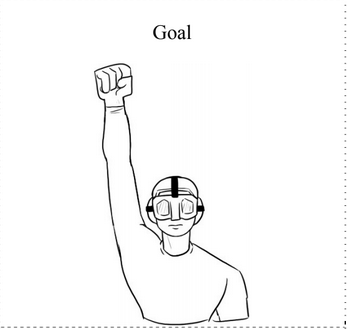
\includegraphics[scale=0.8]{goalScoredSignal}
    \end{center}
\end{frame}

\begin{frame}{Basic signals}
    \begin{center}
        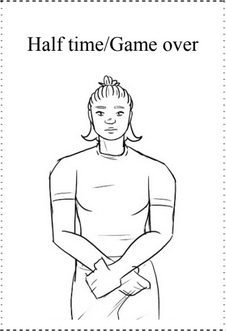
\includegraphics[scale=0.8]{endOfPeriodSignal}
    \end{center}
\end{frame}

\begin{frame}{Basic signals}
    \begin{center}
        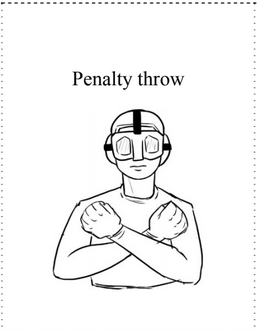
\includegraphics[scale=0.8]{penaltyShotSignal}
    \end{center}
\end{frame}

\begin{frame}{Basic signals}
    \begin{center}
        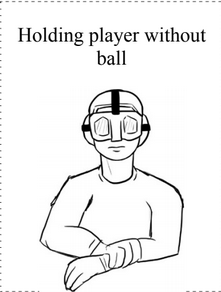
\includegraphics[scale=0.8]{holdingSignal}
    \end{center}
\end{frame}

\begin{frame}{Basic signals}
    \begin{center}
        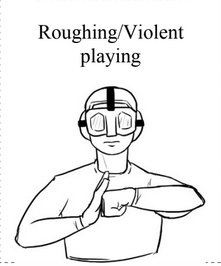
\includegraphics[scale=0.8]{violentGameSignal}
    \end{center}
\end{frame}

\begin{frame}{Basic signals}
    \begin{center}
        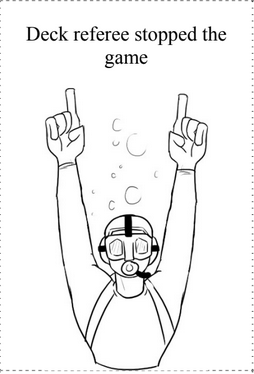
\includegraphics[scale=0.8]{surfaceRefSignal}
    \end{center}
\end{frame}

\begin{frame}{Basic signals}
    \begin{center}
        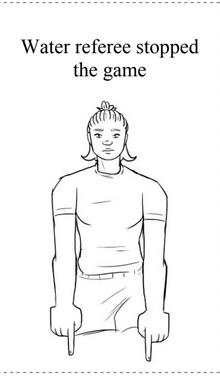
\includegraphics[scale=0.8]{waterRefSignal}
    \end{center}
\end{frame}

\begin{frame}{Basic signals}
    \begin{center}
        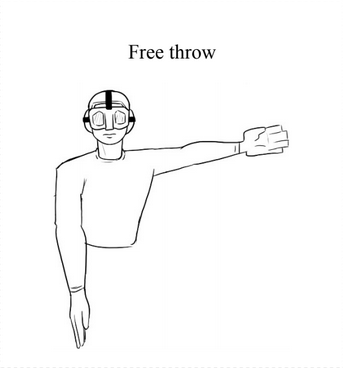
\includegraphics[scale=0.8]{freeThrowSignal}
    \end{center}
\end{frame}

\begin{frame}{Free throw signal}
    The most important signal:
    \begin{enumerate}
        \item Used very often
        \item Indicates next action
        \item Cannot be omitted
    \end{enumerate}
\end{frame}

\begin{frame}{Free throw signal}
    How to signal:
    \begin{enumerate}
        \item Extended arm towards goal to \textbf{attack}
        \item Extended arm towards point to start

              \pause{}

        \item Forming an ``\textbf{L}'' shape \pause{} $\leftarrow$ You must move
    \end{enumerate}
\end{frame}

\begin{frame}{Free throw signal}
    Where should a free throw be started?

    \begin{enumerate}
        \item Foul in team's half $\rightarrow$ Half-way
        \item Foul within 3 meters of basket $\rightarrow$ 3 meters away from basket
        \item Anywhere else $\rightarrow$ Where foul happened
        \item Always in the center of the playing area
    \end{enumerate}
\end{frame}

\subsection{Escalations}

\begin{frame}{Referee attitude}
    The referees are \textbf{responsible} for the match

    When players complain:

    \begin{enumerate}
        \item Players opinions are biased
        \item Don't be intimidated
        \item Be skeptical
        \item If unsure, \textbf{ask}
    \end{enumerate}
\end{frame}

\begin{frame}{Where do you start?}
    Free throws are your bread and butter

    \pause{}

    But you don't always need to start there
\end{frame}

\begin{frame}{When to escalate?}
    Always use your \textbf{best judgement} first.

    \pause{}

    Some example situations:

    \begin{enumerate}
        \item Continuous rough play
        \item Showing contempt
        \item Ignoring calls
        \item Unsportsman behaviour
        \item Continuous questioning
    \end{enumerate}
\end{frame}

\begin{frame}{Warnings}
    \begin{center}
        Used for repeated behaviour

        They \textbf{do not} accumulate

        Can be awarded to the team
    \end{center}
\end{frame}

\begin{frame}{2-minute penalty}
    Used when:

    \begin{enumerate}
        \item Warned foul repeats $\leftarrow$ Including team fouls
        \item Foul was severe
    \end{enumerate}
\end{frame}

\begin{frame}{2-minute penalty}
    Procedure:

    \begin{enumerate}
        \item Penalized player must sit in penalty bench
        \item Replacement is not allowed in
        \item 10 seconds left $\rightarrow$ Lift arm
        \item Time is up $\rightarrow$ Lower arm
    \end{enumerate}
\end{frame}

\begin{frame}{2-minute penalty}
    \begin{center}
        Goal scored against + numerical disadvantage $\rightarrow$ Longest running dismissed
    \end{center}
\end{frame}

\begin{frame}{2 + 2 time penalty}
    \begin{enumerate}
        \item 2 full time penalties
        \item Start one after the other
        \item Dismissed independently
        \item Automatic warning for expulsion
    \end{enumerate}
\end{frame}

\begin{frame}{Expulsion from match}
    \begin{enumerate}
        \item Player must leave pool
        \item 5-minute penalty for team
        \item No numerical disadvantage
        \item Player misses next match
        \item Must be reported to jury
    \end{enumerate}
\end{frame}

\subsection{Penalty shots}

\begin{frame}{Definition}
    \begin{center}
        One attacker Vs. One defender for 45 seconds
    \end{center}
\end{frame}

\begin{frame}{When do they happen}
    \begin{tabular}{ll}
        \parbox{0.5\textwidth} { During a game:

            \begin{enumerate}
                \item Any foul that would \textbf{prevent a goal from being scored}
                \item Always carries a 2-minute time penalty
            \end{enumerate}
        }
         &
        \parbox{0.5\textwidth} { Penalty shootout:

            \begin{enumerate}
                \item Drawn match that requires decision
                \item 3 each (+1 until decision)
                \item No repeated attackers
                \item No repeated defenders
            \end{enumerate}
        }
    \end{tabular}
\end{frame}

\begin{frame}{Refereeing / Surface}
    \begin{tabular}{ll}
        \parbox{0.5\textwidth} {
            \begin{center}
                Before starting
            \end{center}
            \begin{enumerate}
                \item Defender over goal
                \item Attacker in middle
                \item Referees ready
            \end{enumerate}
        }
         &
        \parbox{0.5\textwidth} {
            \begin{center}
                During shot
            \end{center}
            \begin{enumerate}
                \item Keep track of time
                \item Ideally use an alarm
                \item End in the surface
            \end{enumerate}
        }
    \end{tabular}
\end{frame}

\begin{frame}{Referreing / Water}
    \begin{center}
        \textbf{Positioning} is crucial \pause{}

        Keep eyes on the goal and both players
    \end{center}
\end{frame}

\begin{frame}{Refereeing / Water}
    Fouls around the goal

    \begin{enumerate}
        \item Attack on gear
        \item Grabbing basket
        \item Goalkeeper reaching out
    \end{enumerate}

    \pause{}

    You can play \textbf{attacker advantage} during a penalty
\end{frame}

\begin{frame}{Penalty shot outcomes}
    During a game:

    \begin{description}
        \item[Shot defended:] Same as start of period
        \item[Goal scored:] Same as regular goal scored
        \item[Attacker fouls:] Shot defended
        \item[Defender fouls:] Defender 2-minute time penalty + repeat penalty shot
    \end{description}
\end{frame}

\begin{frame}{Penalty shot outcomes}
    In shootout:

    \begin{description}
        \item[Shot defended:] Other team attacks
        \item[Goal scored:] Other team attacks
        \item[Attacker fouls:] Shot defended
        \item[Defender fouls:] Defender misses next shot + repeat penalty shot
    \end{description}
\end{frame}

\subsection{Advantage rule and delayed call}

\begin{frame}{Definition}
    \begin{center}
        Foul happens \pause{}
        $\rightarrow$ \textbf{Wait} \pause{}
        $\rightarrow$ Call based on \textbf{advantage}
    \end{center}
\end{frame}

\begin{frame}{Importance}
    Why is this important? \pause{}

    \begin{enumerate}
        \item Prevents dull games
        \item Avoids teams taking advantage of fouling
        \item Guarantees a more fluid and fair game
    \end{enumerate}

    \pause{}

    \begin{center}
        These \textbf{must} be most of your calls
    \end{center}
\end{frame}

\begin{frame}{Precautions}
    \begin{center}
        Never use when there is a \textbf{safety concern}
    \end{center}
\end{frame}

\begin{frame}{Some considerations}
    A couple things to keep in mind:

    \begin{itemize}
        \item Doesn't affect call order \pause{}
        \item It is \textbf{not optional} \pause{}
        \item Only \textbf{before} play is stopped
    \end{itemize}
\end{frame}

\begin{frame}{The end}
    \begin{center}
        Any questions?
    \end{center}
\end{frame}

\end{document}